\documentclass[a4paper,11pt]{article}
\usepackage{amsmath, amssymb}
\usepackage{enumitem} % For custom lists
\usepackage{fancyhdr} % For header
\usepackage{graphicx} % For including images if needed


\setlength{\parindent}{0pt}
\setlength{\parskip}{1em}


\pagestyle{fancy}
\fancyhf{}
\fancyhead[L]{Introduction to ADS - Exercise Sheet 1}
\fancyhead[R]{Fabian Ibanez Avila \\ 7047016}


\title{Exercise Sheet 1 Solutions}
\author{ Fabian Ibanez Avila \\ 7047016}
\date{\today}

\begin{document}
	
	\maketitle
	
	\section*{Exercise 1: Missing Number}
	
	\begin{figure}[htpb]
		\centering
		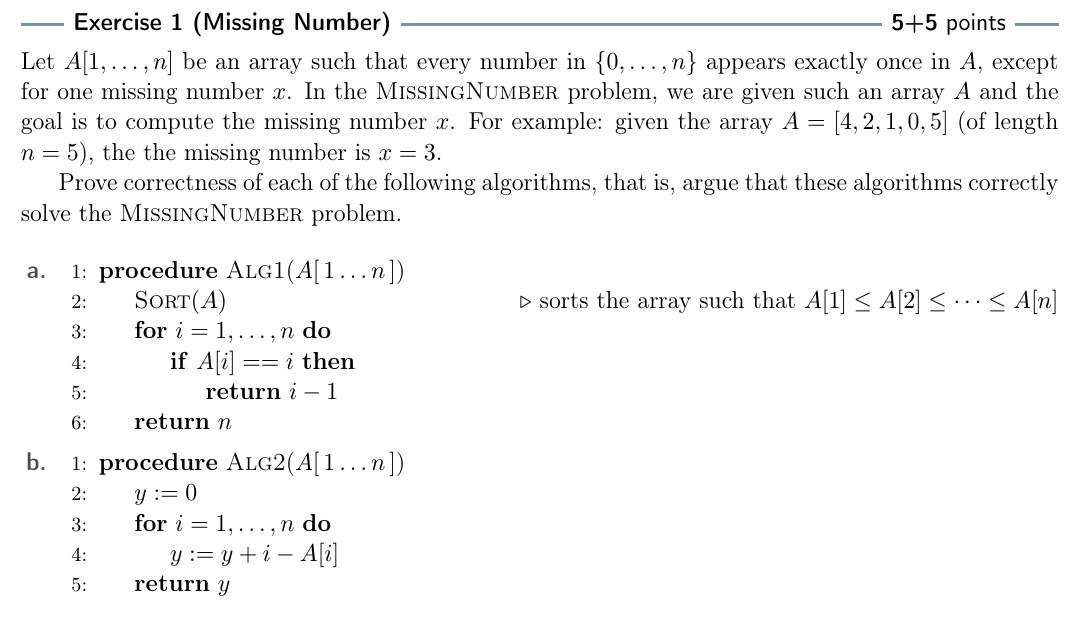
\includegraphics[width=\columnwidth]{/home/fabian/Documents/3. Semester/Introduction to Algorithms and Data Structures/Exercise IADS/Exercise Sheet 1/Ex1.png}
	\end{figure}
	
	\subsection*{Algorithm a}
	\textbf{Correctness Proof:} \\
	The algorithm a is correct. The algorithm first sorts the array into a increasing order. Afterwards, the process of finding the missing number is divided into two different cases. 
	\begin{itemize}
		\item Case 1: The missing number is NOT the last number. 
		\subitem In the sorted algorithm, a number is skipped. As a result, once the for loop arrives to the i index where the number is skipped, the number that should be there is actually the next one. This is exactly what the condition A[i] == i checks. If the condition is true, then the index minus one is returned ( since the index starts at 1 and the sequence at 0 ).
		\item Case 2: The missing number is the last number.
		\subitem The size of the array is n while the size of all possible numbers that could be missing is n+1. Therefore, the array cannot contain all the possible numbers. This means that if the sorted array is a sequence without skipped numbers, the condition inside the for loop will never be triggered. Thus, finally, it should return n ( since the index starts at 1 and the sequence at 0 ).
	\end{itemize}
	
	\subsection*{Algorithm b}
	\textbf{Correctness Proof:} \\
	The algorithm b is correct. To show its correctness, based on the code provided, I will write y as an explicit formula based on the length of the array n and the missing number x. \\
	\[
	y = \sum_{i=1}^{n}i - (\sum_{i=0}^{n}i - x)
	\]
	The first sum of the formula represents the sum of the indices done in the for loop (starting from 0 and ending in n). \\
	Then, the expression inside the parenthesis represents the elements of the array. The sum represents the sum of all the possible elements that the array can contain(from 0 to n), while x is the missing number from the array. By subtracting x from this sum of all possible numbers, we get the sum of all the elements inside the array A. \\
	Now, let us simplify it, so it can become obvious why the code is correct:
	\begin{align*}
		y &= \sum_{i=1}^{n}i - (\sum_{i=0}^{n}i - x) \Leftrightarrow y = \sum_{i=1}^{n}i - (0 + \sum_{i=1}^{n}i - x) \\
		y &= \sum_{i=1}^{n}i - \sum_{i=1}^{n}i + x 	\\
		y &= x 	\\
	\end{align*}
	
	Thus, y is indeed the missing number (that is returned).

	\newpage
	
	\section*{Exercise 2: Polynomial Evaluation}
	
	\begin{figure}[htpb]
		\centering
		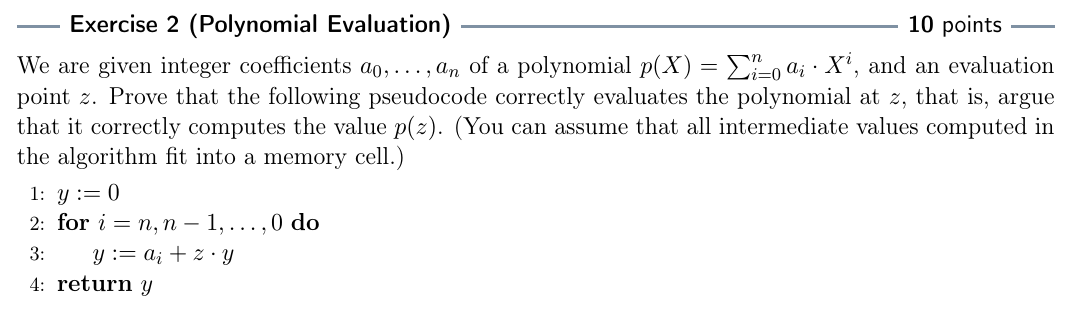
\includegraphics[width=\columnwidth]{/home/fabian/Documents/3. Semester/Introduction to Algorithms and Data Structures/Exercise IADS/Exercise Sheet 1/Ex2.png}
	\end{figure}
	
	\subsection*{Solution}
	
	To show the correctness of the program, I will transform \(y\) from its recursive form to an explicit form:
	
	\[
	y = a_0 + (a_1 +(a_2 + ... + (a_{n-1} + a_n*z)*...)*z)*z
	\] 
	
	After this transformation, we notice that the form of \(y\) is actually the same as the Horner's method for polynomials (view in MFI II). Thus, we obtain pseudocode that correctly computes the values of \(p(z)\).
	
	\newpage
		
	\section*{Exercise 3: Polynomial Evaluation}
	
	\begin{figure}[htpb]
		\centering
		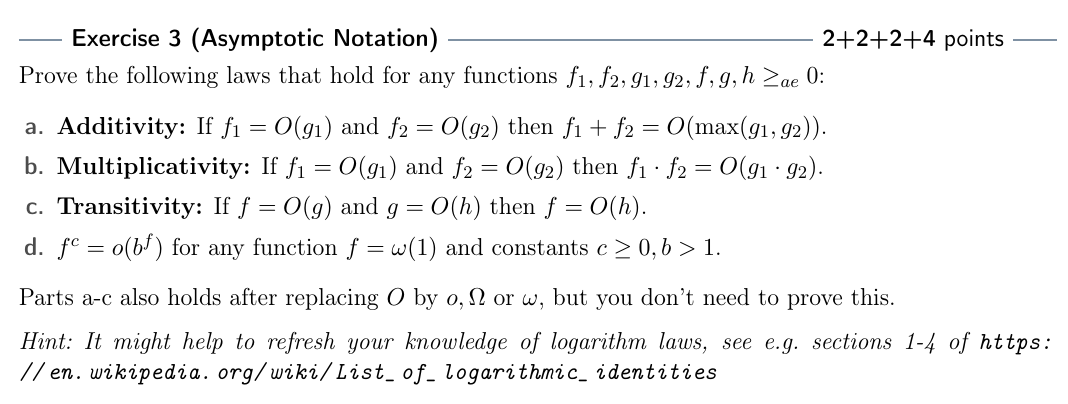
\includegraphics[width=\columnwidth]{/home/fabian/Documents/3. Semester/Introduction to Algorithms and Data Structures/Exercise IADS/Exercise Sheet 1/Ex3.png}
	\end{figure}
	
	\subsection*{Solution}
	
	\subsubsection*{a)}
	
	We know that:
	\begin{align*}
		f_1 \in O(g_1) \Leftrightarrow O(g_1) := \{f_1 \ge_{ae} 0 | \exists c_1 > 0 : f_1 \le_{ae} c_1*g_1  \} \\
		f_2 \in O(g_2) \Leftrightarrow O(g_2) := \{f_2 \ge_{ae} 0 | \exists c_2 > 0 : f_1 \le_{ae} c_2*g_2  \} 
	\end{align*}
	Then, assume \(f_1 =  O(g_1)\) and \(f_2 = O(g_2)\), then:
	\[
		f_1 + f_2 \le_{ae} c_1*g_1 + c_2*g_2 \le_{ae} (c_1 + c_2)*(g_1 + g_2) \le_{ae} (c_1 + c_2)*\text{max}(g_1,g_2 
	\]
	Now, if we set the constant c to \(c_1 + c_2\), we obtain the form of the claim. Thus the claim is correct.
	
	\subsection*{b)}
	
	Following the same logic as before, assume \(f_1 =  O(g_1)\) and \(f_2 = O(g_2)\), then:
	\[
	f_1*f_2 \le_{ae} c_1*g_1 * c_2*g_2 \Leftrightarrow (c_1*c_2)*(g_1*g_2)
	\]
	By setting \(c := c_1 * c_2\), we obtain the same form as in the claim. Thus, property is indeed correct.
	\newpage
	
	\subsection*{c)}
	
	We know that:
	\begin{align*}
		f \in O(g) \Leftrightarrow O(g) := \{f \ge_{ae} 0 | \exists c_g > 0 : f \le_{ae} c_g*g  \} \\
		g \in O(h) \Leftrightarrow O(h) := \{g \ge_{ae} 0 | \exists c_h > 0 : h \le_{ae} c_h*h \} 
	\end{align*}
	Now, assume \(f \in O(g)\) and \(g \in O(h)\), then:
	\[
		f \le_{ae} c_g*g \le c_h*h \Leftrightarrow f \le_{ae} c_h*h
	\]
	Thus, the claim is proved.
	
	\subsection*{c)}
	
	
	
	\section*{Exercise 4: Asymptotic Growth}
	
	\begin{figure}[htpb]
		\centering
		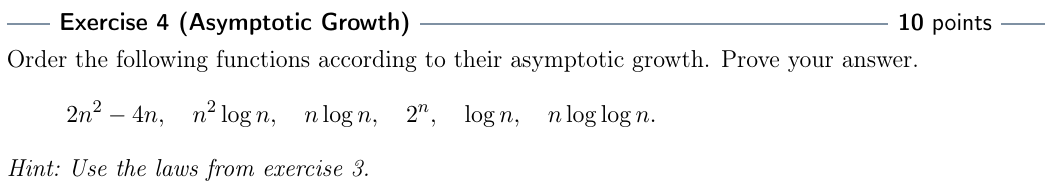
\includegraphics[width=\columnwidth]{/home/fabian/Documents/3. Semester/Introduction to Algorithms and Data Structures/Exercise IADS/Exercise Sheet 1/Ex4.png}
	\end{figure}
	
	\subsection*{Solution}
	\textbf{Solution:} \\
	\[ 
	log (n) \le_{ae} n * log (log(n)) \le_{ae} n*log(n)   \le_{ae} 2n^2 - 4n \le_{ae} n^2 * log(n)\le_{ae} 2^n
	\]
	First, from multiplicativity, we notice that \(log(n) \le_{ae} n\) and that \(1 \le_{ae} log(log(n)) \), then \(log(n) \le_{ae} n * log(log(n)) \). \\
	Second, we know that \(log n \le_{ae} n\) and as log is an increasing function, we can apply the function to both sides without changing the growth, so \(log(log n) \le_{ae} log(n)\). Now, by applying  multiplicativity with \(n\), we obtain \(n log(log(n)) \le_{ae} n log(n)\). \\
	Third, following multiplicativity once again with \(log(n) \le_{ae} n\), it results in \(n* log(n)\le_{ae} n^2\). Then by more multiplicativity and additivity, we obtain \(n*log(n) \le_{ae} 2n^2 - 4n\) 
	Fourth, we notice from additivity that \(2n^2 - 4n \in O(2n^2)\) and from this, that \(2 \le_{ae} log(n)\). So, from multiplicativity, we can observe that  \(2n^2 \le_{ae} n^2*log\), this means that \(2n^2 - 4n  \le_{ae} n^2*log(n)\)\\
	Last, from the last property of the exercise 3, we can notice that $n^2 \in 2^n$, this means that $n^2$ is asymptotically much smaller than $2^n$. Thus,$n^2 * log(n) \in 2^n$
	
	
	
\end{document}
